%%%%%%%%%%%%%%%%%%%%%%%%%%%%%%%%%%%%%%%%%%%%%%%%%%%%%%%%%%
%   Autoren:
%   Prof. Dr. Bernhard Drabant
%   Prof. Dr. Dennis Pfisterer
%   Prof. Dr. Julian Reichwald
%%%%%%%%%%%%%%%%%%%%%%%%%%%%%%%%%%%%%%%%%%%%%%%%%%%%%%%%%%

%%%%%%%%%%%%%%%%%%%%%%%%%%%%%%%%%%%%%%%%%%%%%%%%%%%%%%%%%%
%	ANLEITUNG: 
%   1. Ersetzen Sie firmenlogo.jpg im Verzeichnis img
%   2. Passen Sie alle Stellen im Dokument an, die mit 
%      @stud 
%      markiert sind
%%%%%%%%%%%%%%%%%%%%%%%%%%%%%%%%%%%%%%%%%%%%%%%%%%%%%%%%%%

%%%%%%%%%%%%%%%%%%%%%%%%%%%%%%%%%%%%%%%%%%%%%%%%%%%%%%%%%%
%	ACHTUNG: 
%   Für das Erstellen des Literaturverzeichnisses wird das 
%   modernere Paket biblatex in Kombination mit biber 
%   verwendet - nicht mehr das ältere Paket BibTex!
%
%   Bitte stellen Sie Ihre TeX-Umgebung entsprechend ein (z.B. TeXStudio): 
%   Einstellungen --> Erzeugen --> Standard Bibliographieprogramm: biber
%%%%%%%%%%%%%%%%%%%%%%%%%%%%%%%%%%%%%%%%%%%%%%%%%%%%%%%%%%

\documentclass[fontsize=12pt,BCOR=5mm,DIV=12,parskip=half,listof=totoc,
               paper=a4,toc=bibliography,pointlessnumbers]{scrreprt}
               
               %toc=listof,listof=entryprefix,
               
\makeindex

%% Elementare Pakete, Konfigurationen und Definitionen werden geladen (gegebenenfalls anpassen)
% !TEX root =  master.tex

%%%%%%%%%%%%%%%%%%%%%%%%%%%%%%%%%%%%%%%%%%%%%%%%%%%%%%%%%%%%%%%%%%
%	ANLEITUNG: 
% Passen Sie gegebenenfalls alle Stellen im Dokument an, die mit 
% @stud 
% markiert sind.
%%%%%%%%%%%%%%%%%%%%%%%%%%%%%%%%%%%%%%%%%%%%%%%%%%%%%%%%%%%%%%%%%%

%%
%% @stud
%%
%% LANGUAGE SETTINGS
\usepackage[ngerman]{babel} 	        % german language
\usepackage[german=quotes]{csquotes} 	% correct quoting using \enquote{}
%\usepackage[english]{babel}          % english language
%\usepackage{csquotes} 	              % correct quoting using \enquote{}
\usepackage{eurosym}
\usepackage{makeidx}                  % allows index generation
\usepackage{listings}	                %Format Listings properly
\usepackage{lipsum}                   % Blindtext
\usepackage{graphicx}       
\usepackage{tabularx}                          % use various graphics formats
\usepackage[german]{varioref}
\usepackage{caption}	                % better Captions
\usepackage{booktabs}                 % nicer Tabs
\usepackage[hidelinks=true]{hyperref} % keine roten Markierungen bei Links
\usepackage{fnpct}                    % Correct superscripts 
\usepackage{calc}                     % Used for extra space below footsepline, in particular
\usepackage{array}
\usepackage{acronym}
\usepackage{algorithm}
\usepackage{algpseudocode}
\usepackage{setspace}
\usepackage{tocloft}
\usepackage{makecell}
\usepackage{hhline}

\usepackage{longtable}
\usepackage{svg}
\usepackage{amssymb}

%Benedikt
\usepackage{xltabular}
\usepackage{amsmath}


% Davids Abschnitt
\usepackage{geometry}
\usepackage{pdflscape}
\usepackage{wrapfig}

%% Schriftarten- und Zeichenpakete
\usepackage[T1]{fontenc}
\usepackage[utf8]{inputenc}

%%
%% @stud
%%
%%	FONT SELECTION: Schriftarten und Schriftfamilie
%%%%%%%%%%%%%
%% SCHRIFTART
%%%%%%%%%%%%%
% 0) without decomment: normal font families 
% ...
% 1) Latin Modern 
\usepackage{lmodern}        
% 2) Times 
%\usepackage{mathptmx}         
% 3) Helvetica
%\usepackage[scaled=.92]{helvet} 
%%%%%%%%%%%%%%%%%%
%%	SCHRIFTFAMILIE
%%%%%%%%%%%%%%%%%%
% ohne Serifen
\renewcommand*{\familydefault}{\sfdefault}
\addtokomafont{disposition}{\sffamily}
%
% mit Serifen
%\renewcommand*{\familydefault}{\rmdefault}
%\addtokomafont{disposition}{\rmfamily}
%
% Typewriter
%\renewcommand*{\familydefault}{\ttdefault}
%\addtokomafont{disposition}{\ttfamily}

%%
%% @stud
%%
%% Uncomment the following lines to support hard URL breaks in bibliography 
%\apptocmd{\UrlBreaks}{\do\f\do\m}{}{}
%\setcounter{biburllcpenalty}{9000}% Kleinbuchstaben
%\setcounter{biburlucpenalty}{9000}% Großbuchstaben

%%
%% @stud
%%
%% FOOTNOTES: Count footnotes over chapters
%% \counterwithout{footnote}{chapter}

%	ACRONYMS
\makeatletter
\@ifpackagelater{acronym}{2015/03/20}
{\renewcommand*{\aclabelfont}[1]{\textbf{{\acsfont{#1}}}}}{}
\makeatother

%	LISTINGS
% @stud: ggf. Namen/Text anpassen (englisch)
\renewcommand{\lstlistingname}{Quelltext} 
\renewcommand{\lstlistlistingname}{Quelltextverzeichnis}
\lstset{numbers=left,
	numberstyle=\tiny,
	captionpos=b,
	basicstyle=\ttfamily\small}

%	ALGORITHMS
% @stud: ggf. Namen/Text anpassen (englisch)
\renewcommand{\listalgorithmname}{Algorithmenverzeichnis}
\floatname{algorithm}{Algorithmus}

%	PAGE HEADER / FOOTER
%	Warning: There are some redefinitions throughout the master.tex-file!  DON'T CHANGE THESE REDEFINITIONS!
\RequirePackage[automark]{scrlayer-scrpage}
%alternatively with separation lines: \RequirePackage[automark,headsepline,footsepline]{scrlayer-scrpage}

\renewcommand{\chaptermarkformat}{}
\RedeclareSectionCommand[beforeskip=0pt]{chapter}
\clearpairofpagestyles

%\ifoot[\rule{0pt}{\ht\strutbox+\dp\strutbox}DHBW Mannheim]{\rule{0pt}{\ht\strutbox+\dp\strutbox}DHBW Mannheim}
\ofoot[\rule{0pt}{\ht\strutbox+\dp\strutbox}\pagemark]{\rule{0pt}{\ht\strutbox+\dp\strutbox}\pagemark}
\ohead{\headmark}

\newcommand{\TitelDerArbeit}[1]{\def\DerTitelDerArbeit{#1}\hypersetup{pdftitle={#1}}}
\newcommand{\AutorDerArbeit}[1]{\def\DerAutorDerArbeit{#1}\hypersetup{pdfauthor={#1}}}
\newcommand{\Firma}[1]{\def\DerNameDerFirma{#1}}
\newcommand{\Kurs}[1]{\def\DieKursbezeichnung{#1}}
\newcommand{\Abteilung}[1]{\def\DerNameDerAbteilung{#1}}
\newcommand{\Studiengangsleiter}[1]{\def\DerStudiengangsleiter{#1}}
\newcommand{\WissBetreuer}[1]{\def\DerWissBetreuer{#1}}
\newcommand{\FirmenBetreuer}[1]{\def\DerFirmenBetreuer{#1}}
\newcommand{\Bearbeitungszeitraum}[1]{\def\DerBearbeitungszeitraum{#1}}
\newcommand{\Abgabedatum}[1]{\def\DasAbgabedatum{#1}}
\newcommand{\Matrikelnummer}[1]{\def\DieMatrikelnummer{#1}}
\newcommand{\Studienrichtung}[1]{\def\DieStudienrichtung{#1}}
\newcommand{\ArtDerArbeit}[1]{\def\DieArtDerArbeit{#1}}
\newcommand{\Literaturverzeichnis}{Literaturverzeichnis}

\newcommand{\DavidsGeileTabellen}[1]{
	\pagebreak
	
	\newgeometry{left=1cm,right=1cm,top=1cm,bottom=1cm}
	\begin{landscape}

		
		\thispagestyle{empty}
		
		\begin{table}
			\begin{tabularx}{27.7cm}{c c p{3cm} X c c c p{2.5cm} c X}
				\textbf{ID} &\textbf{Risikotyp}&\textbf{Titel} &\textbf{Beschreibung} &\textbf{WSK} &\textbf{Stärke} &\textbf{Risiko} &\textbf{Problem Zeitpunkt} &\textbf{MKat} &\textbf{Maßnahme}\\\toprule
				#1
			\end{tabularx}
		\end{table}


	\end{landscape}
	\restoregeometry
}

\newcommand{\settingBibFootnoteCite}{
	\setlength{\bibparsep}{\parskip}		  % Add some space between biblatex entries in the bibliography
	\addbibresource{bibliography.bib}	    % Add file bibliography.bib as biblatex resource
	\DefineBibliographyStrings{ngerman}{andothers = {{et\,al\adddot}},}
}

\newcommand{\setTitlepage}{
	% !TEX root =  master.tex
% @stud: ggf. Namen/Text anpassen (englisch)
\begin{titlepage}
\begin{minipage}{\textwidth}
		\vspace{-2cm}
		\noindent \hfill 
\includegraphics{\imagedir/logo.jpg}
\end{minipage}
\vspace{1em}
%\sffamily
\begin{center}
	{\textsf{\large Duale Hochschule Baden-W\"urttemberg Mannheim}}\\[4em]
	{\textsf{\textbf{\large{\DieArtDerArbeit}arbeit}}}\\[6mm]
	{\textsf{\textbf{\Large{}\DerTitelDerArbeit}}} \\[1.5cm]
	{\textsf{\textbf{\large{}Studiengang Wirtschaftsinformatik}}\\[6mm]
	\textsf{\textbf{Studienrichtung \DieStudienrichtung}}}\vspace{15em}
	
	\begin{minipage}{\textwidth}
		\begin{tabbing}
		Wissenschaftliche(r) Betreuer(in): \hspace{0.85cm}\=\kill
		Verfasser: \> \DerAutorDerArbeit \\[1.5mm]
		Matrikelnummer: \> \DieMatrikelnummer \\[1.5mm]
%		Firma: \> \DerNameDerFirma  \\[1.5mm]
%		Abteilung: \> \DerNameDerAbteilung \\[1.5mm]
		Kurs: \> \DieKursbezeichnung \\[1.5mm]
		Studiengangsleiter: \> \DerStudiengangsleiter \\[1.5mm]
		Dozent: \> \DerWissBetreuer \\[1.5mm]
%		Firmenbetreuer(in): \> \DerFirmenBetreuer \\[1.5mm]
		Bearbeitungszeitraum: \> \DerBearbeitungszeitraum\\[1.5mm]
%		alternativ:\\[1.5mm]
%		Eingereicht: \> \DasAbgabedatum	
		\end{tabbing}
	\end{minipage}
\end{center}
\end{titlepage}
	\pagenumbering{roman} % Römische Seitennummerierung
	\normalfont	
}

\newcommand{\initializeText}{
	\clearpage
	\ihead{\chaptername~\thechapter} % Neue Header-Definition
	\pagenumbering{arabic}           % Arabische Seitenzahlen
}

\newcommand{\initializeBibliography}{
	\ihead{}
	\printbibliography[title=\Literaturverzeichnis] 
	\cleardoublepage
}

\newcommand{\initializeAppendix}{
	\appendix
	\ihead{}
	\cftaddtitleline{toc}{chapter}{Anhang}{}
}


%%
%% @stud
%%
%% PERSÖNLICHE ANGABEN (BITTE VOLLSTÄNDIG EINGEBEN zwischen den Klammern: {...})
%%
%Aktuelle Data Science Entwicklungen 2
\ArtDerArbeit{Gruppen} % "Bachelor" oder "Projekt" wählen
\TitelDerArbeit{Soccer Twos RL}
\AutorDerArbeit{Eric Echtermeyer, Lasse Friedrich, \\[1.5mm] \>Benedikt Prisett, David Schäfer}
%\Abteilung{<Ihre Abteilung>}
%\Firma{<Ihre Firma>}
\Kurs{WWI-21-DSA}
\Studienrichtung{Data Science}
\Matrikelnummer{6373947, 9924680, 5709658, 7086451}
\Studiengangsleiter{Prof. Dr.-Ing. habil. Dennis Pfisterer}
\WissBetreuer{Dr. Manuel Zeise}
%\FirmenBetreuer{<Ihr(e) Firmenbetreuer(in)>}
\Bearbeitungszeitraum{22.05.2024 -- 15.07.2024}

%%
%% @stud
%%
%% BIBLIOGRAPHY (@stud: Bibliographie-Stil wählen - Position und Indizierung)
%%  Auswahl zwischen: 
%%   NUMERIC Style
%%   IEEE Style
%%   ALPHABETIC Style
%%   HARVARD Style
%%   CHICAGO Style 
%%   (oder eigenen zulässigen Stil wählen) 
%%
%%%%%%%%%%%%%
%% Zitierstil
%%%%%%%%%%%%%
% NUMERIC Style - e. g. [12]
\newcommand{\indextype}{numeric} 
%
% IEEE Style - numeric kind of style 
%\newcommand{\indextype}{ieee} 
%
% ALPHABETIC Style - e. g. [AB12]
%\newcommand{\indextype}{alphabetic} 
%
% HARVARD Style 
%\newcommand{\indextype}{apa} 
%
% CHICAGO Style 
%\newcommand{\indextype}{authoryear}
%
%%%%%%%%%%%%%%%%%%%%%%
%% Position des Zitats
%%%%%%%%%%%%%%%%%%%%%%
\newcommand{\position}{inline} 
%
% (!!) FOOTNOTE POSITION NOT RECOMMENDED IN MINT DOMAIN:
%\newcommand{\position}{footnote}

%% Final: Setzen des Zitierstils und der Zitatposition
\usepackage[backend=biber, autocite=\position, style=\indextype]{biblatex} 	
\settingBibFootnoteCite

%%
%% Definitionen und Commands
%%
\newcommand{\abs}{\par\vskip 0.2cm\goodbreak\noindent}
\newcommand{\nl}{\par\noindent}
\newcommand{\mcl}[1]{\mathcal{#1}}
\newcommand{\nowrite}[1]{}
\newcommand{\NN}{{\mathbb N}}
\newcommand{\imagedir}{img}

\makeindex

\begin{document}

\setTitlepage

%%%%%%%%%%%%%%%%%%%%%%%%%%%%%%%%%%%
% EHRENWÖRTLICHE ERKLÄRUNG
%
% @stud: ewerkl.tex bearbeiten
%
%% !TEX root =  master.tex
\clearpage
\chapter*{Ehrenwörtliche Erklärung}

% Wird die folgende Zeile auskommentiert, erscheint die ehrenwörtliche
% Erklärung im Inhaltsverzeichnis.

% \addcontentsline{toc}{chapter}{Ehrenwörtliche Erklärung}
Ich versichere hiermit, dass ich die vorliegende Seminararbeit mit dem Titel ``\textit{\DerTitelDerArbeit}'' selbstständig verfasst und 
keine anderen als die angegebenen Quellen und Hilfsmittel benutzt habe. Ich versichere zudem, dass die eingereichte elektronische 
Fassung mit der gedruckten Fassung übereinstimmt.

\vspace{3cm}
Ort, Datum \hfill \DerAutorDerArbeit
 
%\cleardoublepage  
%%%%%%%%%%%%%%%%%%%%%%%%%%%%%%%%%%%

%%%%%%%%%%%%%%%%%%%%%%%%%%%%%%%%%%%
% SPERRVERMERK
%
% @stud: nondisclosurenotice.tex bearbeiten
%
%% !TEX root =  master.tex
\chapter*{Sperrvermerk}

\begin{center}
\fbox{
		\begin{minipage}{33em}
			\textbf{Ein Sperrvermerk sollte nur bei berechtigtem Bedarf gesetzt werden!\\[10pt] 
				Beachten Sie, dass mit Sperrvermerk	versehene Arbeiten nicht für weitere wissenschaftliche Zwecke 
				außerhalb des Firmenkontextes oder zur Publikation verwendet werden dürfen.\\[10pt]
				Wir empfehlen, wenn m\"oglich, auf den Sperrvermerk zu verzichten.\\[10pt]
				Besprechen Sie diese Problematik mit Ihrer Firma!}
		\end{minipage}
}
\end{center}

(Mustertext) Der Inhalt dieser Arbeit darf weder als Ganzes noch in Auszügen Personen außerhalb des Prüfungsprozesses 
und des Evaluationsverfahrens zugänglich gemacht werden, sofern keine anders lautende Genehmigung der Ausbildungsstätte vorliegt. 

\cleardoublepage
 
%\cleardoublepage
%%%%%%%%%%%%%%%%%%%%%%%%%%%%%%%%%%%

%%%%%%%%%%%%%%%%%%%%%%%%%%%%%%%%%%%
%	KURZFASSUNG
%
% @stud: acknowledge.tex bearbeiten
%
%% !TEX root =  master.tex
\chapter*{Danksagung}

Hier können Sie eine Danksagung schreiben. 



%\cleardoublepage 
%%%%%%%%%%%%%%%%%%%%%%%%%%%%%%%%%%%

%%%%%%%%%%%%%%%%%%%%%%%%%%%%%%%%%%%
% VERZEICHNISSE und ABSTRACT
%
% @stud: ggf. nicht benötigte Verzeichnisse auskommentieren/löschen
%
\tableofcontents
\cleardoublepage

% Abbildungsverzeichnis
\phantomsection
\addcontentsline{toc}{chapter}{\listfigurename}
\listoffigures
\cleardoublepage

%	Tabellenverzeichnis
\phantomsection
\addcontentsline{toc}{chapter}{\listtablename}
\listoftables
\cleardoublepage

%	Listingsverzeichnis / Quelltextverzeichnis
%\lstlistoflistings
%\cleardoublepage

% Algorithmenverzeichnis
%\listofalgorithms
%\cleardoublepage

% Abkürzungsverzeichnis
% @stud: acronyms.tex bearbeiten
% !TEX root =  master.tex
\clearpage
\chapter*{Abkürzungsverzeichnis}	
\addcontentsline{toc}{chapter}{Abkürzungsverzeichnis}

\begin{acronym}[XXXXXXX]
	\acro{RL}{Reinforcement Learning}
	\acro{MARL}{Multi Agent Reinforcement Learning}
	\acro{ML}{Machine Learning}
\end{acronym} 
\cleardoublepage

%	Kurzfassung / Abstract
% @stud: abstract.tex bearbeiten
% !TEX root =  master.tex
\chapter*{Abstract}
Hier steht das Abstarct.

Das ist ein Zitat \cite{sutton_reinforcement_1998}. 
\cleardoublepage

%%%%%%%%%%%%%%%%%%%%%%%%%%%%%%%%%%%%%%%%%%%%%%%%%%%%%%%%%%%%%%%%%%%%%%%%%%%%%%%%%%%%%%%%%%
% KAPITEL UND ANHÄNGE
%
% @stud:
%   - nicht benötigte: auskommentieren/löschen
%   - neue: bei Bedarf hinzufügen mittels input-Komman do an entsprechender Stelle einfügen
%%%%%%%%%%%%%%%%%%%%%%%%%%%%%%%%%%%%%%%%%%%%%%%%%%%%%%%%%%%%%%%%%%%%%%%%%%%%%%%%%%%%%%%%%%

\initializeText
\onehalfspacing

%%%%%%%%%%%%%%%%%%%%%%%%%%%%%%%%%%%
% KAPITEL
%
% @stud: einzelne Kapitel bearbeiten und eigene Kapitel hier einfügen
%
% Einleitung
%% !TEX root =  master.tex
\chapter{Einleitung}

\nocite{*}

Dieses Kapitel enthält die Einleitung mit ihren verschiedenen Abschnitten/Sections und Unterabschnitten.

\section{Beispiel Abschnitt: \LaTeX-Installation}

Zur Verwendung von \LaTeX-Installation einer Distribution z.~B.~TeXLive, MikTex etc.~sowie eines Editors z.~B.~TeXStudio, TeXnicCenter etc.~notwendig.

Installieren Sie zun\"achst die Distribution und anschließend den Editor. Beim ersten Start des Editors \"offnet sich ein 
Konfigurationsassistent, der zun\"achst nach dem Pfad der installierten Distribution fragt. 

Nach der Installation können k\"onnen Einstellungen z.~B.~f\"ur einen PostScript-Viewer gemacht werden. 
Dieser Schritt kann ohne Weiteres \"ubersprungen werden. Entscheidend sind die Einstellungen f\"ur den pdf-Viewer. 

Jetzt kann \LaTeX~verwendet werden. Um die Ausgabe eines Dokumentes zu erzeugen, muss das Dokument kompiliert werden (Ausgabe >
Aktives Dokument > Erstellen und betrachten).

\subsection{Beispiel Unterabschnitt: Aufbau eines \LaTeX-Dokuments}

Ein \LaTeX-Dokument besteht in der Regel aus folgenden Komponenten:
\begin{itemize}
	\item Pr\"aambel
	\item Titelseite
	\item Textteil
\end{itemize}

\subsection{Beispiel Unterabschnitt auf zweiter Ebene: Pr\"aambel}
In der Pr\"aambel werden global die Einstellungen f\"ur das gesamte Dokument definiert. Hierbei k\"onnen z.~B.~die Seitenr\"ander, 
der Zeilenabstand oder auch die Sprache f\"ur die Silbentrennung festgelegt werden. In der ersten Zeile eines jeden Dokumentes wird dabei
immer die zu verwendende Klasse festgelegt. Standardm\"aßig kann hier die Artikel-Klasse gew\"ahlt werden:

\texttt{\textbackslash documentclass[12pt,titlepage]\{article\}}

In den eckigen Klammern wird dabei u.a. die Standardschriftgr\"o\ss e f\"ur das gesamte Dokument festgelegt. 

Au\ss erdem werden in der Pr\"aambel die f\"ur das Dokument ben\"otigten Pakete festgelegt. Gebr\"auchlich sind vor allem folgende Pakete:
{\texttt{
\begin{itemize}
	\item \textbackslash usepackage[ngerman]\{babel\}
	\item \textbackslash usepackage[latin1]\{inputenc\}
	\item \textbackslash usepackage\{color\}
	\item \textbackslash usepackage[a4paper]\{geometry\}
	\item \textbackslash usepackage\{amssymb\}
	\item \textbackslash usepackage\{amsthm\}
	\item \textbackslash usepackage\{graphicx\}
\end{itemize}
}

Im vorliegenden Fall werden die Pakete in der Konfigurationsdatei \texttt{config.tex} festgelegt, deren Inhalt durch 
\texttt{\textbackslash input\{config\}} in das Hauptdokument \texttt{master.tex} inkludiert wird.

\subsubsection{Beispiel Unterabschnitt auf zweiter Ebene: Titelseite}

Nachdem die Dokumenten-Klasse und die zu verwendenden Pakete festgelegt worden sind,
folgt die Titelseite. Da die Titelseite bereits Teil des eigentlichen Dokuments ist, muss ihr
unbedingt der Befehl \texttt{\textbackslash begin\{document\}} vorausgehen. Am Ende des Dokuments sollte der Befehl
\texttt{\textbackslash end\{document\}} gesetzt werden. Alles was nach diesem Befehl steht, wird vom Compiler nicht mehr beachtet.

\section{Noch ein Beispiel-Abschnitt}

Der Textteil beinhaltet nun den eigentlichen Text des Dokuments.


% mehrere Grundlagen- und Forschungs-Kapitel
% !TEX root = master.tex
\chapter{Einführung} \label{chapter:1}
%Darstellung des Problems, der Umgebung mit Regeln/ Dynamik und ggf. Vereinfachungen.

Im Rahmen dieser Gruppenarbeit mit dem Ziel der Implementierung von erlernten \ac{RL} Verfahren wurde sich für das ``Soccer Twos''-Problem \cite[p. 15]{juliani2020} entschieden. Es handelt sich hierbei um eine, als Teil des ``Unity \ac{ML} Agents Toolkit'' \cite{juliani2020} veröffentlichte, Umgebung, welche ein vereinfachtes Fußballspiel zwischen zwei Teams mit je zwei Spielern simuliert und somit ein \ac{MARL} Problem darstellt.
Die Entscheidung für dieses \ac{RL}-Problem wurde getroffen, auf Grundlage der geigneten Anwendungsmöglichtkeit von den in der Veranstaltung behandelten Verfahren, sowie den Anspruch auf eine durchaus herausfordernde Aufgabe, welche durch die erhöhte Komplexität des Multi-Agent Problem hier gegeben ist. 

\section{Soccer Twos Umgebung}

Das Unity \ac{ML} Agents Toolkit verfügt über diverse Komponenten um \ac{RL} verwandte Aspekte in Unity-Umgebungen umzusetzen und bietet zudem eine Vielzahl an Beispiel-Umgebungen und Implementierungen von \ac{RL}-Algorithmen, welche es Spieleentwicklern oder Forschern ermöglicht \ac{RL}-Verfahren zu entwicklen und testen. 
Die bereitgestellten Beispielumgebungen zeigen die Einsatzmöglichkeiten des Toolkits durch kleinere Spiele, die größtenteils in einer 3D-Umgebung stattfinden, auf. In den Umgebungen agieren einfache blockförmige und auch komplexere mit Gelenken ausgestattete Agenten, die alleine oder gemeinsam verschiedene Aufgaben lösen müssen. Die Beobachtungsräume dieser Agent sind größtenteils in Vektorform dargestellt sowie in einzellnen Fällen auch visuell und die Aktionsräume sind je nach Spiel entweder diskret oder kontinuierlich. Dies bietet somit eine Ausgangslage für die Anwedung von \ac{RL}-Verfahren in unterschiedlichstem Umfang.

Da das Toolkit mit seinem beträchtlichen Funktionsumfang bereits eine gewisse Komplexität aufweist, wurde entschieden, das Projekt in einer ausschließlich Python-basierten Gymnasium-Umgebung umzusetzen und dementsprechend ein passendes Paket zu nutzen \cite{soccertwos}. Dieses Paket ermöglichte es, die komplette Implementierung in Python durchzuführen und die bereits bekannten Gymnasium-Schnittstellen zu nutzen.

Beim Spiel ``Soccer Twos'' spielen zwei Agenten gemeinsam in einem Team gegen ein weiteres Zweier-Team Fußball. Es handelt sich hierbei um eine 3D-Spielumgebung, die in Abbildung \ref{fig:soccer_twos_3d} dargestellt ist. Das Spielfeld ist mit einer Bande begrenzt, wodurch es kein Aus gibt und das Spiel nicht unterborchen wird. Zu Beginn eines Spiels liegt der Ball in der Mitte des Feldes, und die beiden Teams starten auf ihrer jeweiligen Seite des Spielfelds. Die Agenten sind nicht unbedingt in der Lage, komplexe bzw. sehr präzise Schüsse auszuführen, sondern passen und schießen lediglich, indem sie einfach gegen den Ball laufen. Es ist das Ziel jedes Teams, den Ball in das gegnerische Tor zu befördern und gleichzeitig das eigene Tor zu schützen.

\begin{figure}[h]
	\centering
	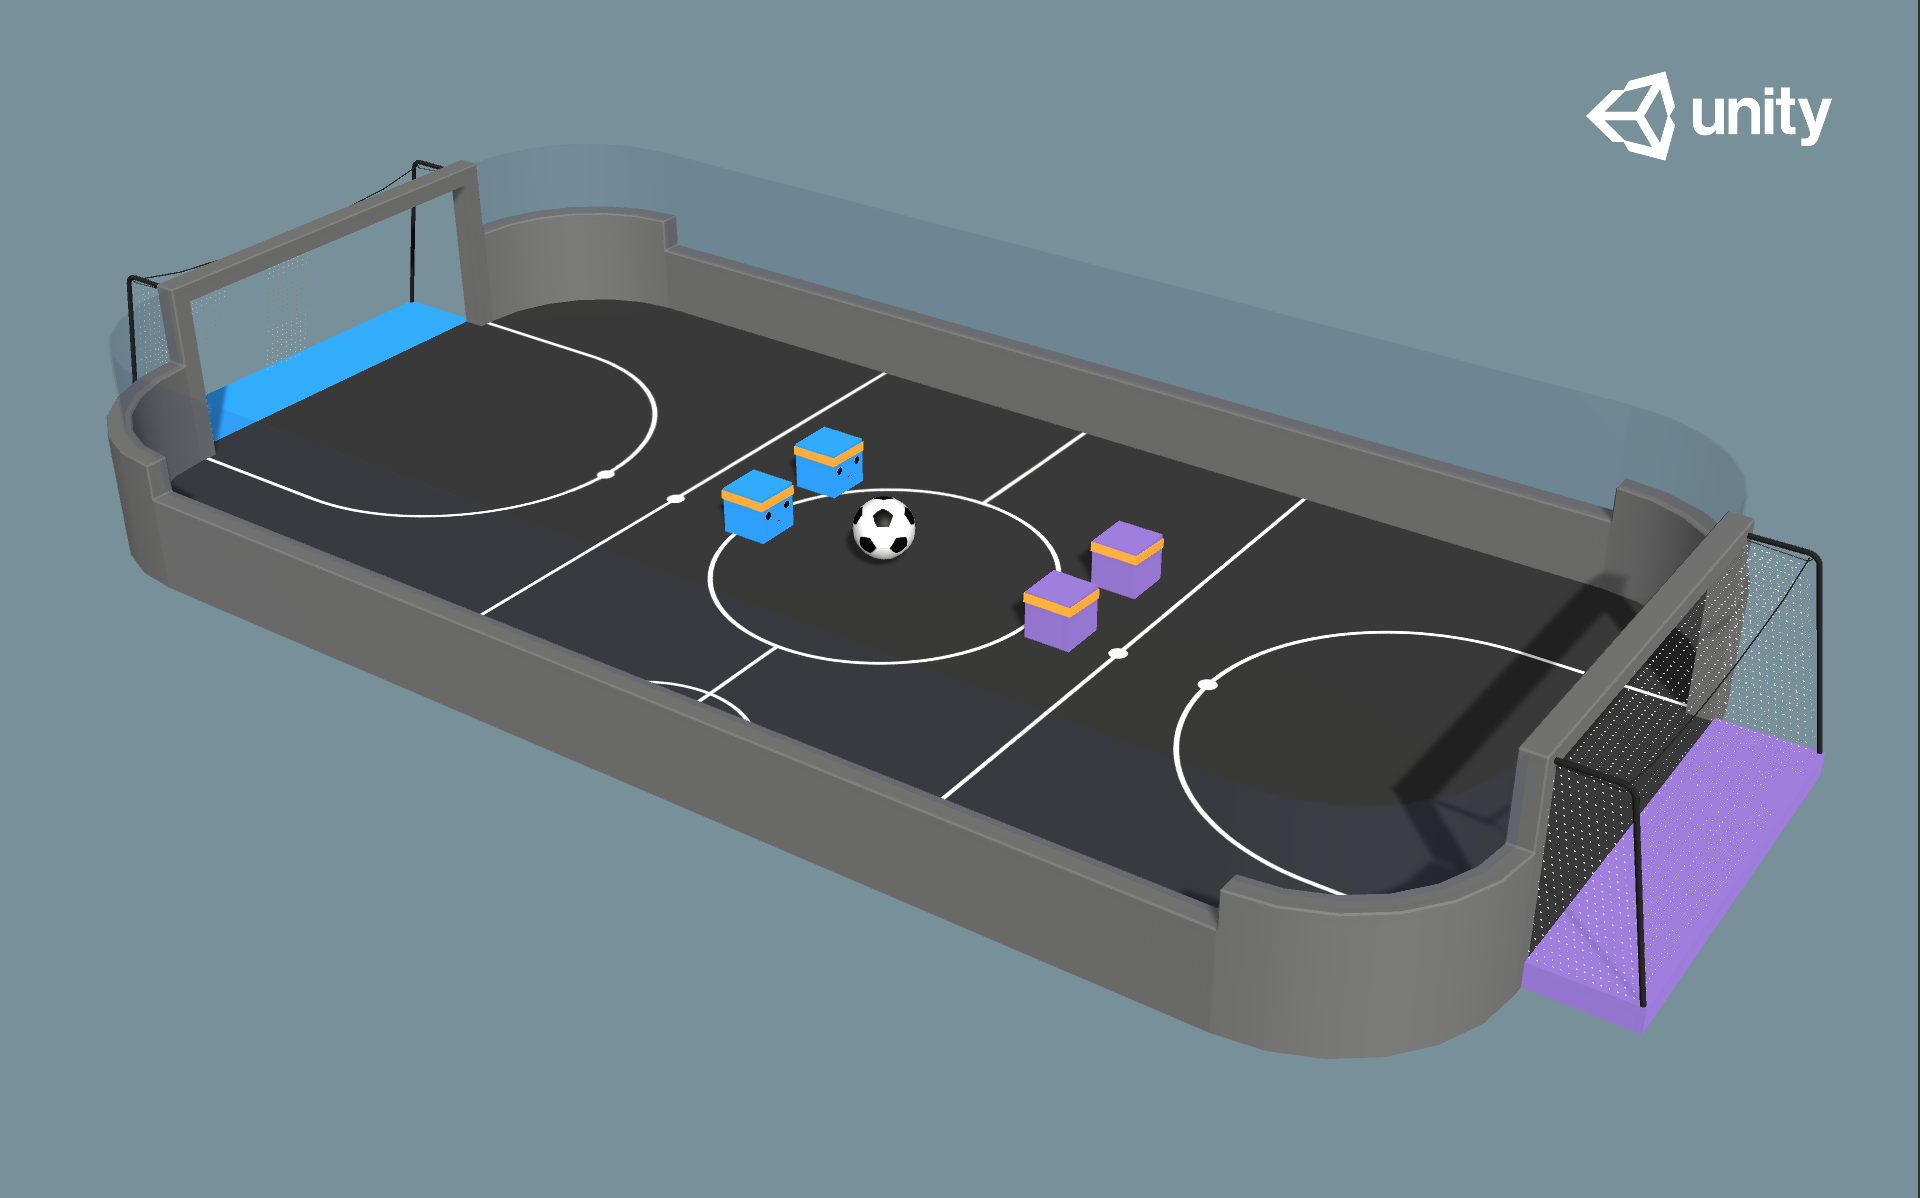
\includegraphics[width=\textwidth]{img/soccer_twos.png}
	\caption{Die visualisierte 3D-Spielumgebung von ``Soccer Twos'' des Unity \ac{ML}-Agents Toolkits. Die zwei Teams in Blau und Pink mit jeweils zwei blockförmigen Agenten stehen sich gegenüber, während der Fußball im Mittelkreis liegt. \cite{juliani2020}}
	\label{fig:soccer_twos_3d}
\end{figure}

Der Aktionsraum eines Agents ist diskret und umfasst die drei Dimensionen ``Vorgehen oder Zurückgehen'', ``Rechtsgehen oder Linksgehen'' sowie ``Linksdrehen oder Rechtsdrehen''. Für jede Dimension kann ein Wert aus \(\{0,1, 2\}\) gewählt werden, wobei \(0\) für keine Ansteuerung auf dieser Dimension steht, \(1\) für die zuerst genannte Aktion und \(2\) für die zweite. Zum einfachen Vorwärtsgehen sieht der Aktionsvektor somit wie folgt aus: \([1, 0, 0]\) oder schräg Vorwärts und Links: \([1, 2, 0]\). Es gibt somit 27 mögliche diskrete Aktionen.
Die Aktionen werden während eines Spiels für alle Agents gleichzeitig definiert und in einem 4-elementigen Dictionary übergeben.

Der Beobachtungsraum besteht aus einem Vektor mit 336 Dimensionen. Diese Dimensionen ergeben sich aus mehreren Strahlen (sogenannten Ray-Casts), die die Umgebung eines Agents abtasten. Konkret werden 11 Strahlen nach vorne ausgesendet, die einen Bereich von 120° abdecken, und 3 Strahlen nach hinten, die einen Bereich von 90° abdecken. Jeder dieser Strahlen kann 6 verschiedene Objekttypen erkennen und die Entfernung zu diesen Objekten messen. Um Bewegungsabfolgen zu erkennen, werden die Daten von drei aufeinanderfolgenden Beobachtungen zusammengeführt. %todo: klären wie die Dokumentation auf 336 kommt

Jedes Spiel wird entweder für 1000 Iterationen oder bis ein Tor erzielt wird gespielt. Die Belohnungsfunktion verleiht eine positive Belohnung von \(1 - \text{akkumulierte Zeitstrafe}\), wenn ein Tor erzielt wird. Zu Beginn einer Episode wird die Zeitstrafe auf \(0\) gesetzt und dann bei jedem Update um \( \frac{1}{\text{max Schritte}} \). Diese Berechnung der Belohnung trägt somit dazu bei, dass vor allem das schnelle Schießen eines Tores unterstützt wird.  Erhält ein Team ein Gegentor, wird eine negative Belohnung von \(-1\) verhängt, um so die Verteidigung des eigenen Tores anzureizen.
%todo: erweiterung beschreiben (lasse fragen)


\section{Multi Agent \acl{RL}}

Bei ``Soccer Twos'' handelt es sich um ein \ac{MARL}-Problem, welches ein Teilgebiet des normalen \ac{RL} darstellt. \ac{MARL} befasst sich mit Umgebungen, in denen mehrere Agenten agieren und somit auch miteinander interagieren können und sich durch ihre Aktionen gegenseitig beeinflussen.

Diese Umgebungen sind dezentral oder zentral aufgebaut. In einer dezentralen Umgebung wird jeder Agent alleine und unabhängig von den anderen Agenten trainiert, was bedeutet, dass jeder weiterhin seine eigene Belohnungsstruktur, Beobachtungen und Aktionen hat und im Lernprozess keine Informationen zwischen den Agenten geteilt werden. Dies hat den Vorteil, dass jeder Agent alleine trainiert werden kann und die anderen Agenten einfach als Teil der Umgebung wahrnimmt. Eine derartige Struktur hat jedoch den großen Nachteil, dass sie eine nicht-stationäre Umgebung erzeugt, auf die viele \ac{RL}-Algorithmen angewiesen sind.
In einer zentralen Umgebung hingegen gibt es eine übergeordnete Struktur, welche die Beobachtungen und Belohnungen aller Agenten sammelt und verarbeitet. Dadurch kann eine einzige gemeinsame Policy erlernt werden und das Wissen wird zwischen den Agenten geteilt. \cite{Tan:1993} %https://web.media.mit.edu/~cynthiab/Readings/tan-MAS-reinfLearn.pdf
%Zentral und dezentral https://huggingface.co/learn/deep-rl-course/en/unit7/multi-agent-setting

Neben der Art der Umgebung lässt sich weiter zwischen zwei Interaktionstypen der Agenten unterscheiden \cite{10.1007/11691839_1}. In kooperativen Umgebungen agieren mehrere Agenten, um eine gemeinsame Belohnung zu maximieren. Es ist also das Ziel, dass die Agenten zusammen eine Aufgabe lösen und sich gegenseitig unterstützen. In konfrontativen Umgebungen treten mehrere Agenten gegeneinander an und versuchen, ihre eigene Belohnung zu maximieren, während die Belohnung des Gegners minimiert wird.
Weiter ist es möglich, dass diese beiden Arten auch in gemischter Form auftreten und es somit in einer Umgebung sowohl kooperative Agenten gibt, die aber konfrontativ gegenüber anderen auftreten. Genau um eine solche gemischte Umgebungsform handelt es sich auch bei dem ``Soccer Twos''-Problem. Zwei Agenten eines Teams spielen gemeinsam kooperativ gegen ein anderes Team, welches einen konfrontativen Gegner darstellt.


%ggf. noch so sagen das meisten rl probleme in der vergangenheit nur einen agent betrachtet haben aber marl für realität etc. viel interessanter ist und daher in der vergangeheit jetzt mehr erforscht wurde aber eben auch komplexer ist.


% !TEX root = master.tex
\chapter{Methoden} \label{chapter:2}
%Übersicht der angewandten Methoden, Beschreibung einer Baseline-Methode.

Zum lösen des \enquote{Soccer Twos} Problem wurden im Rahmen dieser Gruppenarbeit verschiedene, unterschiedlich komplexe, Methoden angewendet. Zunächst wurde eine einfach Baseline entwickelt mit der die späteren \ac{RL}-Algorithmen verglichen werden können. Im Folgenden wurde als erstes ein alleiniger \ac{RL}-Agent trainiert, mit dem Ziel ein Tor zu erziehlen. Anschließend wurde versucht dies nun auf das \ac{MARL}-Problem mit dem Training mehrerer Agents zu erweitern.

\section{Baseline}

Um eine adäquate Vergleichbarkeit und Bewertung der implementierten \ac{RL}-Verfahren zu ermöglichen, wurde zunächst eine einfache Baseline-Methode für das \enquote{Soccer Twos}-Problem entworfen und implementiert. Diese Baseline beruht auf den zwei Verhaltensweisen, \enquote{Verteidigungsmodus} und \enquote{Angriffsmodus}, die auf Basis der von der Umgebung bereitgestellten Informationen durchgeführt werden.

Der \enquote{Verteidigungsmodus} wird ausgelöst, sobald sich der Ball auf der Heimseite des Spielfelds befindet und somit die Gefahr für ein Gegentor besteht. Die Agents versuchen in diesem Fall, das eigene Tor zu verteidigen, indem sie sich zwischen das Tor und den Ball bewegen. Dies geschieht, indem sie sich zunächst zum Mittelpunkt zwischen dem Ball und dem Tor drehen und anschließend vorwärts zu diesem Mittelpunkt laufen. Da dies wiederholt ausgeführt wird, bewegen sich die Agents somit zwischen den Ball und das Tor und wehren Schüsse auf das eigene Tor ab.
Der \enquote{Angriffsmodus} wird ausgeführt, sobald der Ball auf die gegnerische Spielfeldseite gelangt und somit ein Angriff auf das gegnerische Tor stattfinden kann. Die Agents drehen sich nun so lange, bis der Winkel zwischen Spieler und Ball kleiner als 30 Grad ist, und laufen dann auf den Ball zu. Befindet sich der Ball jedoch hinter dem Spieler wird die Bewegung angepasst, sodass ein Eigentor verhindert werden kann. Die Idee des \enquote{Angriffsmodus} ist es somit, dass ein Agent alles darauf setzt, einen Schuss durchzuführen und somit ein Tor zu erzielen.

Diese simple Baseline, beruhend auf festen Regeln, ermöglicht ein einfaches Fußballspiel zwischen den Agents, welches nicht besonders komplex und effizient ist, aber ein vereinfachtes Spielgeschehen mit gelegentlichen erfolgreichen Torschüssen oder Abwehraktionen erlaubt. Das Ziel der im Folgenden entwickelten \ac{RL}-Verfahren ist es nun, diese einfache Spielweise zu übertreffen.


\section{Single Agent RL Algorithmen}

Zum Einstieg wurden für das \enquote{Soccer Twos} Problem zunächst einige grundlegende \ac{RL}-Algorithmen angewendet, die sich jedoch nur auf einen Agent beschränken. Es wurde somit eine Vereinfachung vorgenommen und nicht direkt das deutlich komplexere \ac{MARL} Problem, bei welchem mehrere Agents trainiert werden müssen, betrachtet, um zu Beginn die allgemeine Machbarkeit und Komplexität des Trainingsprozesses zu untersuchen. Im Rahmen dieser Vereinfachung werden weiter vier Agents und ein Ball zu Start des Spiels zufällig auf dem Feld platziert, jedoch kann sich nur einer dieser Agents bewegen und wird trainiert. 

Insgesamt wurden zwei Off-Policy- und zwei On-Policy-Methoden für das vereinfachte, auf einen Agent beschränkte Problem angewendet. 
Bei Off-Policy-Verfahren wird die Policy, die der Agent erlernt, unabhängig von jener behandelt, die das Verhalten während des Lernprozesses bestimmt. Das bedeutet, dass die gesammelten Erfahrungen nicht nur von der aktuellen Policy des Agenten abhängen, sondern auch von einer anderen Policy stammen können.
Bei On-Policy-Methoden hingegen erlernt ein Agent die gleiche Policy, die auch während des Lernprozesses verwendet wird, um Aktionen zu bestimmen. Der Agent bewertet und optimiert diese Policy direkt anhand der durch diese Policy generierten Erfahrungen.

%DQN
Ein typischer Ansatz zum lösen von \ac{RL}-Problemen ist der \textbf{\ac{DQN}} Algorithms. Es handelt sich hierbei um eine Off-Policy Methode welche das Q-Learning mit tiefen neuronalen Netzwerken kombiniert, um optimale Handlungsstrategien zu erlernen. Der Kern des \ac{DQN} besteht darin, eine Q-Funktion zu approximieren, die den erwarteten zukünftigen Belohnungswert für eine gegebene Aktion in einem bestimmten Zustand angibt. %hier könnte mathematische funktion aber paper sonst schnell zu lang
Durch kontinuierliches Training und Anpassung der Gewichte des neuronalen Netzwerks kann der Agent somit lernen, optimale Aktionen zu wählen, die langfristig zu höheren Belohnungen führen \cite{mnih2013}. 
%Eine Erweiterung dieses Verfahrens stellt der \ac{DDQN} Algorithmus dar.  Dieser soll die Überschätzung von Q-Werten verringern, indem zwei separate Netzwerke verwendet werden. Eines dieser Netze übernimmt die Auswahl der Aktionen und das andere ist für die Bewertung dieser zuständig. Diese Trennung ermöglicht eine stabilere und genauere Schätzung der Q-Werte, was zu einem robusteren Lernprozess führt.

%PG
Ein ebenfalls verbreitete Off-Policy Methode ist der \ac{PG} Algorithmus, welcher sowohl für kontinuierlichen als auch diskrete Aktionsräume geeignet ist. Bei diesem Verfahren wird direkt eine Policy-Funktion, in Form eines Neuronalen Netzes, erlernt, die angibt, welche Aktion in einem gegebenen Zustand ausgeführt werden soll.
Eine Erweiterung dieser Methode stellt der \ac{DPG} und auch \textbf{\ac{DDPG}} Algorithmus dar. Diese verwenden zwei Netzwerke: ein Actor-Netzwerk, das die Policy darstellt und Aktionen auswählt, und ein Critic-Netzwerk, das den Q-Wert der ausgewählten Aktionen schätzt. Es wird somit die Stabilität und Effizienz des Lernens verbessert und bietet vor allem bei komplexeren Aufgaben in kontinuierlichen Aktionsräumen Vorteile. 
%DDPG noch detailierter?
%ggf. nochmal darauf eingehen das wir das trotz diskreten Aktionsraum nutzen und warum

%PPO
Ein weiterer bedeutender Ansatz in diesem Bereich ist die \textbf{\ac{PPO}} Methode. \ac{PPO} ist ein On-Policy Algorithms, gehört zur Familie der \ac{PG} Methoden und zielt darauf ab, die Instabilitäten und hohen Varianzen traditioneller \ac{PG} Algorithmen zu reduzieren. Dies wird durch die Einführung eines speziellen Clipping-Mechanismus erreicht, der die Updates der Policy innerhalb eines bestimmten Bereichs hält. Dieser Mechanismus stellt sicher, dass die Änderungen an der Policy während des Trainings nicht zu drastisch sind, wodurch ein stabilerer und effizienterer Lernprozess gewährleistet wird \cite{SchulmanWDRK17}.

%A2C
Ein weiterere On-Policy Methode ist der \textbf{\ac{A2C}} Algorithmus.
\ac{A2C} kombiniert Elemente der Actor-Critic-Architektur mit Vorteilsschätzungen (Advantage-Funktion). Der Kern der \ac{A2C} Methode besteht somit wie bei den vorherigen Methoden ebenfalls aus einem Policy- und Critic-Netzwerk. Zusätzlich wird jedoch noch eine Advantage-Funktion erlernt, welche den Vorteil einer Aktion in einem bestimmten Zustand im Vergleich zum durchschnittlichen erwarteten Wert aller möglichen Aktionen in diesem Zustand, bestimmt. Durch die Berechnung des Advantage-Werts kann der Algorithmus genauer die Unterschiede zwischen guten und schlechten Aktionen erfassen, was zu effizienteren Policy-Updates führt \cite{MnihBMGLHSK16}.

%SAC
%Ein weiterere Methode ist der \ac{SAC} Algorithms. \ac{SAC} kombiniert Elemente der Actor-Critic-Architektur mit einer Entropiemaximierung, um eine explorativere und robustere Policy zu erlernen. Der Kern der \ac{SAC} Methode besteht somit ebenfalls darin, sowohl ein Policy-Netzwerk (Actor) als auch ein Q-Netzwerk (Critic) zu erlernen. Der wesentliche Unterschied zu anderen Methoden liegt jedoch in der Maximierung der Entropie der Policy. Dies bedeutet, dass der Agent nicht nur darauf abzielt, die Belohnung zu maximieren, sondern auch die Unsicherheit seiner Entscheidungen zu berücksichtigen und somit eine vielfältigere Aktionsauswahl zu ermöglichen. Diese Entropie-Maximierung fördert eine bessere Exploration und verhindert das Verharren in suboptimalen Policys \cite{todo}. 

% NN Struktur
Da die Ansteuerung der Agents, wie zuvor beschrieben, über einen dreielementigen Aktionsvektor mit drei möglichen Werten für jedes Element erfolgt, wurde die Struktur der bei den \ac{RL}-Algorithmen verwendeten neuronalen Netze entsprechend angepasst. Die Ausgabeschicht des Netzwerkes besteht aus neun Neuronen, die in drei Gruppen, welche jeweils eine Bewegungsdimension darstellen, aufgeteilt sind. Innerhalb jeder dieser Gruppen steht je ein Neuron für keine Ansteuerung, die erste mögliche Aktion oder die zweite mögliche Aktion. Die Auswahl der letztendlich durchgeführten Aktion für dieses Element des Aktionsvektors erfolgt durch die Wahl des Maximalwertes innerhalb dieser Gruppe.

%Da die Ansteuerung der Agents, wie zuvor beschrieben, über einen dreielementigen Aktionsvektor mit drei möglichen Werten für jedes Element erfolgt, wurde die Struktur der bei den \ac{RL}-Algorithmen verwendeten neuronalen Netze entsprechend angepasst. Die Ausgabeschicht des Netzwerkes besteht aus neun Neuronen, die in drei Gruppen, welche jeweils eine Bewegungsdimension darstellen, aufgeteilt sind. Innerhalb jeder dieser Gruppen wird ein Softmax angewendet und je ein Neuron steht für keine Ansteuerung, die erste mögliche Aktion. Die Auswahl der letztendlich durchgeführten Aktion für dieses Element des Aktionsvektors erfolgt durch die Wahl des Maximalwertes innerhalb dieser Gruppe.


%Sparse Rewards
Bereits beim Training dieser ersten Algorithmen wurden einige Auffälligkeiten beobachtet. Besonders die Tatschache das in der \enquote{Soccer-Twos}-Umgebung nur relativ selten ein Tor und somit eine Belohnung für den Agenten erziehlt wird führte zu einem sehr langsamen Lernprozess und schlechten Ergebnissen. Da es sich hier somit um eine sogennante \enquote{sparse reward} Umgebung handelt, in welcher die Belohnungen selten und unregelmäßig auftreten, wurde die Behlohnungsfunktion der Agenten angepasst. Neben einer Belohung für ein erzieltes Tor erhalten die Agenten nun fortlaufend einen Belohnung welche auf ihrem Abstand zum Ball baisert. Diese neue Behlohung nimmt \(1\) an, wenn der Abstand zum Ball minimal ist und \(0\) wenn der Abstand maximal, also 32 Einheiten, groß ist. Die neue Belohnungsstruktur der Umgebung kann somit mit folgender Formel zusammengefasst werden:

\[
\text{Belohnung} = \begin{cases} 
	1 - \text{akkumulierte Zeitstrafe} & \text{wenn ein Tor erzielt wird} \\
	-1 & \text{wenn ein Gegentor erzielt wird} \\
	\max\left(0, 1 - \frac{\text{Abstand zum Ball}}{\text{maximaler Abstand}}\right) & \text{sonst}
\end{cases}
\]

Durch diese Anpassung wird der Agent nun angeregt sicher schneller zum Ball zu bewegen und die Wahrscheinlichkeit das er eine sinnvolle Aktion und letztendlich ein Tor erziehlt steigt.

%Stable Baseline
Eine weitere wichtige Entscheidung, die im Laufe des Entwicklungsprozesses getroffen wurde, war die Verwendung der \ac{SB3} Bibliothek \cite{stable-baselines3} für die Implementierung der \ac{PPO} und \ac{A2C} Methoden. Es handelt sich hierbei um eine Open-Scource-Bibliothek welche robuste und effiziente Implementierungen einer Vielzahl an moderneren \ac{RL}-Algorithmen bietet.
Zu Beginn wurden die verschiedenen Verfahren zwar eigenständig implementiert, jedoch stießen diese aufgrund der hohen Komplexität schnell an ihre Grenzen. Durch die Nutzung von \ac{SB3} konnte eine korrekte Implementierung sichergestellt werden. Zudem ermöglicht die Bibliothek den Einsatz fortschrittlicher Optimierungsverfahren und unterstützt Multiprocessing während des Trainings. Dies führte zu einer erheblichen Verbesserung der Trainingszeit und der erzielten Ergebnisse.

\section{Multi Agent Methode}

 Aufbauend auf den bei der Implementierung der vorherigen Methoden gewonnenen Erkenntnissen wurde im Folgenden das \ac{MARL}-Problem betrachtet. Da es sich hierbei um ein großes Themenfeld mit vielen, teils sehr komplexen Methoden handelt und bereits beim Training in einfacheren Single-Agent-Umgebungen einige Herausforderungen auftraten, wurden die Untersuchungen im \ac{MARL}-Bereich auf die Anwendung eines \enquote{competitive self-plays} mit dem \ac{PPO}-Algorithmus beschränkt.
 
 Bei \enquote{competitive self-play} spielt und lernt ein Agent, indem er gegen sich selbst oder eine alternative Version seiner selbst antritt. Im Kontext des \enquote{Soccer-Twos}-Problems wurde eine Population an Agenten erzeugt, die in anfangs zufällig zugeordneten Spielen gegeneinander antreten. Basierend auf diesen Spielen erhalten die Agenten ein Update zu ihrem ELO-Rating, einer Bewertung, die ihre relative Spielstärke widerspiegelt, und sammeln währenddessen individuell Erfahrungen. Nach ihren Spielen werden diese Erfahrungen genutzt, um ihre jeweilige Policy zu aktualisieren. Dieses Verfahren wird wiederholt fortgesetzt, wobei jedoch nun die Zuordnung der Spielgegner aufgrund der ELO-Ratings getroffen wird. Hierdurch kann sichergestellt werden, dass ein Agent gegen einen Gegner auf ähnlichem Niveau antritt und so durch die angemessene Herausforderung des Spiels in der Lage ist, seine eigenen Fähigkeiten iterativ zu verbessern.
% !TEX root = master.tex
\chapter{Anwendung} \label{chapter:3}
%Grafische Darstellung des Lernprozesses, zentraler Ergebnisse und Beispiele der Agenten.

Die in \ref{chapter:2} beschriebenen Methoden erwiesen sich bei ihrer Anwendung auf das ``Soccer-Tows'' Problem als unterschiedliche erfolgreich.


\iffalse %temporär auskommentiert

%Single Agent Methods
\ref{fig:bild} zeigt ein Vergleich der verschiedenen Methoden mit Werten für die angepassten Belohnungsstruktur links und original Belohung (Tor oder Gegentor) für ein Spiel rechts.

\begin{figure}[h]
	\centering
	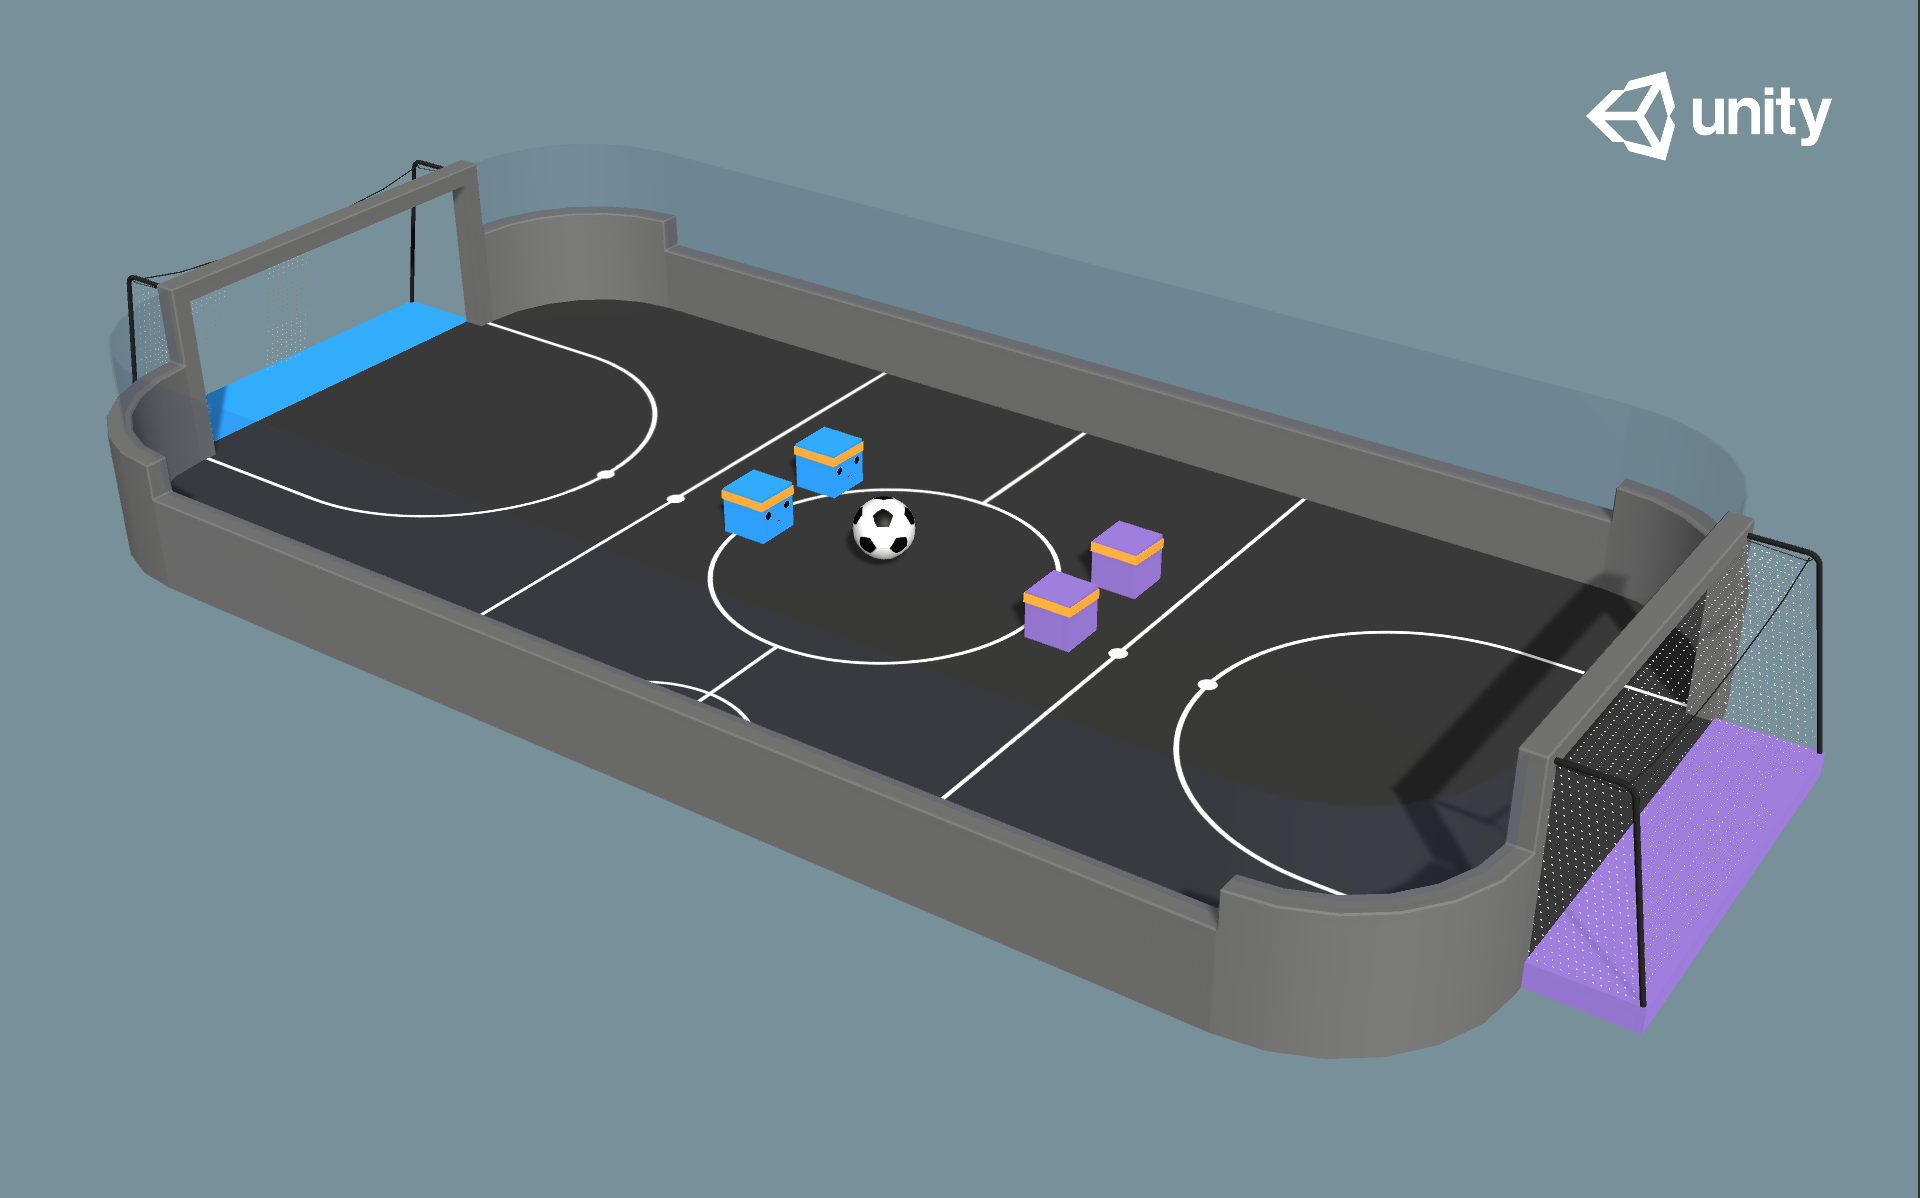
\includegraphics[width=\textwidth]{img/soccer_twos.png}
	\caption{Caption BOXPLOTS}
	\label{fig:bild}
\end{figure}

Es ist zu erkennen, dass die Off-Policy Methoden \ac{XY} und \ac{XY} die schlechtesten Ergenisse liefern. \ac{XY} zeigt einen mit ... einen mitterleren Erfolg. Die besten Ergenisse erziehlt der \ac{PPO} Algorithmus, welcher ... .
Im Vergleich zu der entwickleten Baseline-Methode ist es ersichtlich das .... .


\ref{fig:bild2} stellt .... dar. 

\begin{figure}[h]
	\centering
	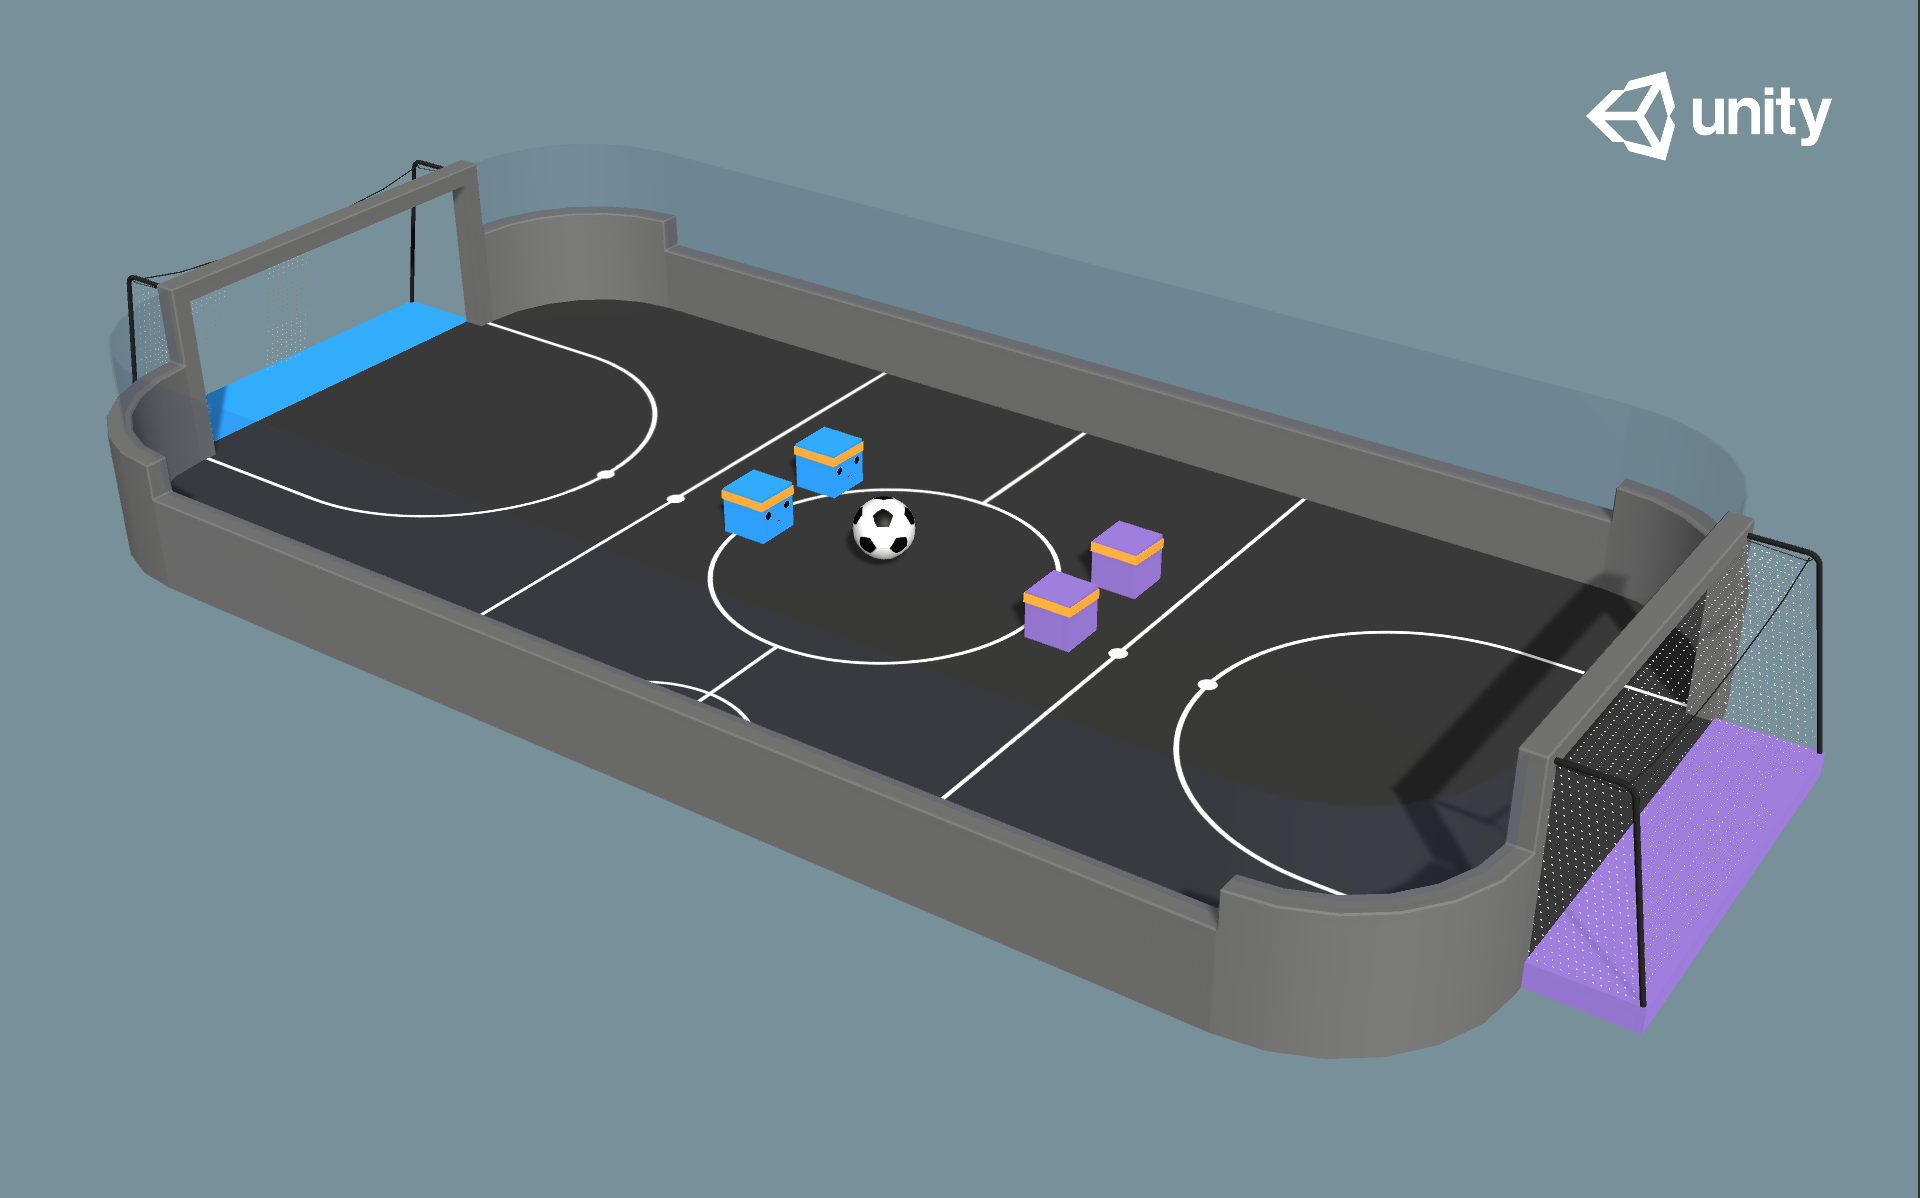
\includegraphics[width=\textwidth]{img/soccer_twos.png}
	\caption{Caption ANDERE GRAFIK}
	\label{fig:bild2}
\end{figure}

Auch diese Darstellung unterstricht die zuvor beschriebenen Erkennisse. (... was hier noch neu rausgelsen wird)


%MARL

Die Anweung des ``competetiv-self play'' Verfahrens für das Mulit-Agent-Szenario ....

\fi
% !TEX root = master.tex
\chapter{Abschluss} \label{chapter:4}
Bewertung und Einordnung der Ergebnisse, Limitierungen der Methoden (z.B. aufgrund begrenzter Computing-Ressourcen), mögliche Erweiterungen.
%\input{chapter5}
%\input{chapter6}
% Fazit und Ausblick
%% !TEX root =  master.tex
\chapter{Zusammenfassung}

\nocite{*}

Dieses Kapitel enthält die Zusammenfassung der Arbeit mit Fazit und Ausblick.

\section{Fazit}

...

\section{Ausblick}

...


%%%%%%%%%%%%%%%%%%%%%%%%%%%%%%%%%%%

%%%%%%%%%%%%%%%%%%%%%%%%%%%%%%%%%%%
% ANHÄNGE
%
% @stud: einzelne Anhänge bearbeiten und eigene Anhänge hier einfügen 
%        die nachfolgenden Zeilen deaktivieren, wenn keine Anhänge verwendet werden
%
%\initializeAppendix
%% !TEX root =  master.tex
\chapter{Beispiel-Anhang: Testanhang}

%% !TEX root =  master.tex
\chapter{Beispiel-Anhang: Noch ein Testanhang}
nochmal: lipsum ...

%%%%%%%%%%%%%%%%%%%%%%%%%%%%%%%%%%%

\singlespacing

%%%%%%%%%%%%%%%%%%%%%%%%%%%%%%%%%%%
% LITERATURVERZEICHNIS
% @stud: Literaturverzeichnis in Datei bibliography.bib anpassen. 
%
% Alternative zu Verwendung von \initializeBibliography: Citavi ...
% (dann \initializeBibliography auskommentieren und eigenes LaTex Coding verwenden)
%
\initializeBibliography
%%%%%%%%%%%%%%%%%%%%%%%%%%%%%%%%%%%

%%%%%%%%%%%%%%%%%%%%%%%%%%%%%%%%%%%
% INDEX
% @stud: ggf. Index auskommentieren, wenn nicht benötigt
%
%\addcontentsline{toc}{chapter}{Index}
%\printindex

\end{document}
